\documentclass[slides,compress]{beamer}
\usepackage{graphicx,amsmath,hyperref}
\usepackage{verbatim}

\usepackage[normalem]{ulem}

\usetheme{default}
\useinnertheme{rectangles}

\title{\huge Recent Developments in xia2}
\subtitle{\large Strubi early 2012 update}

\author{Graeme Winter}
\institute{Diamond Light Source}
\date{1 March 2012}

\begin{document}

\setbeamertemplate{background}{

\includegraphics[width=\paperwidth,height=\paperheight]
{diamond-background.png}
}

\frame{\maketitle}

\frame{
\frametitle{Overview}
\begin{itemize}
\item{CCP4 2012 presentation}
\item{Removal of frame count limitations}
\item{Current state of multi-crystal analysis}
\item{Other developments}
\item{Conclusions \& plans}
\end{itemize}
}

\frame{
\frametitle{Removal of frame count limitations}
\begin{itemize}
\item{Use Aimless in place of Scala}
\item{Use Pointless in place of Reindex\footnote{This is still not as
      efficient as it could be - but it works}}
\item{Run -3daii or -3da}
\item{No more batch limitations}
\end{itemize}
}

\frame{
\frametitle{Example: 20 sweeps from insulin}
\begin{itemize}
\item{Insulin test sample from I04-1}
\item{20 sweeps: 0.2 degree / frame x 900: 18000 images}
\item{Radiation damage very likely}
\item{Substantial variation between data sets}
\item{Processing rather time consuming, use a big workstation}
\end{itemize}
} 

\begin{frame}[fragile]
\begin{verbatim}
High resolution limit          	  1.66	  7.43	  1.66
Low resolution limit           	 55.18	 55.18	  1.70
Completeness                   	100.0	 99.9	100.0
Multiplicity                   	314.3	346.7	262.8
I/sigma                        	 81.7	228.5	  7.6
Rmerge                         	0.106	0.071	5.227
Rmeas(I)                       	0.106	0.071	5.240
Rmeas(I+/-)                    	0.106	0.071	5.247
Rpim(I)                        	0.006	0.004	0.322
Rpim(I+/-)                     	0.008	0.005	0.450
Wilson B factor                	31.457
Total observations             	2982419	44723	180512
Total unique                   	9488	129	687
\end{verbatim}
\end{frame}

\frame{
\frametitle{Effects of Running Aimless}
\begin{itemize}
\item{Output effectively the same as Scala}
\item{SD correction slightly more effective}
\item{C++ not Fortran - no need to recompile for lots of batches}
\item{Parallel (openMP) version in development}
\end{itemize}
}

\frame{
\frametitle{Effects of Running Aimless in xia2}
\begin{itemize}
\item{Since scaling performed by XSCALE very little difference in results}
\end{itemize}
}

\frame{
\frametitle{Current state of multi-crystal analysis}
\begin{itemize}
\item{Developed over ~ 1 year or so}
\item{Hiatus for most of that time}
\item{Still very rough around the edges}
\item{Requires use of XDS processing}
\item{Requires R (at the moment) to generate plot}
\end{itemize}
}

\frame{
\frametitle{Basic principles}
\begin{itemize}
\item{Assume in processing that everything comes from the same
    crystal}
\item{Try to assemble a data set from everything}
\item{Worry about isomorphism in scaling rather than from unit cell
    etc.}
\item{Look at CC's between sweeps as measure of isomorphism}
\item{Scale CC's to ersatz distance as $d = \frac{1}{CC} -
    1$\footnote{Which means you can \emph{interpret} the distances.}}
\end{itemize}
}

\frame{
\frametitle{Basic Usage}
\begin{center}
{\huge
xia2 -3daii /here/are/my/data
}
\end{center}
}

\frame{
\begin{center}
{\huge
Time passes... let's talk about options
}
\end{center}
}

\frame{
\frametitle{Useful options}
\begin{itemize}
\item{-microcrystal - switch to microcrystal mode}
\item{-failover - ignore failure of processing individual sweeps}
\item{-spacegroup - set the spacegroup as e.g. P23}
\item{-cell $a,b,c,\alpha,\beta,\gamma$ - needs -spacegroup}
\item{-min\_images 3 - minimum images to count as a sweep}
\item{-xparm GXPARM.XDS - refined model of experimental geometry}
\end{itemize}
}

\begin{frame}[fragile]
\frametitle{After processing}
\begin{verbatim}
> cd DEFAULT/scale
> x1335 XSCALE.LP
> R --no-save < x1335.R
\end{verbatim}
\end{frame}

\frame{
\frametitle{Results}
\begin{center}
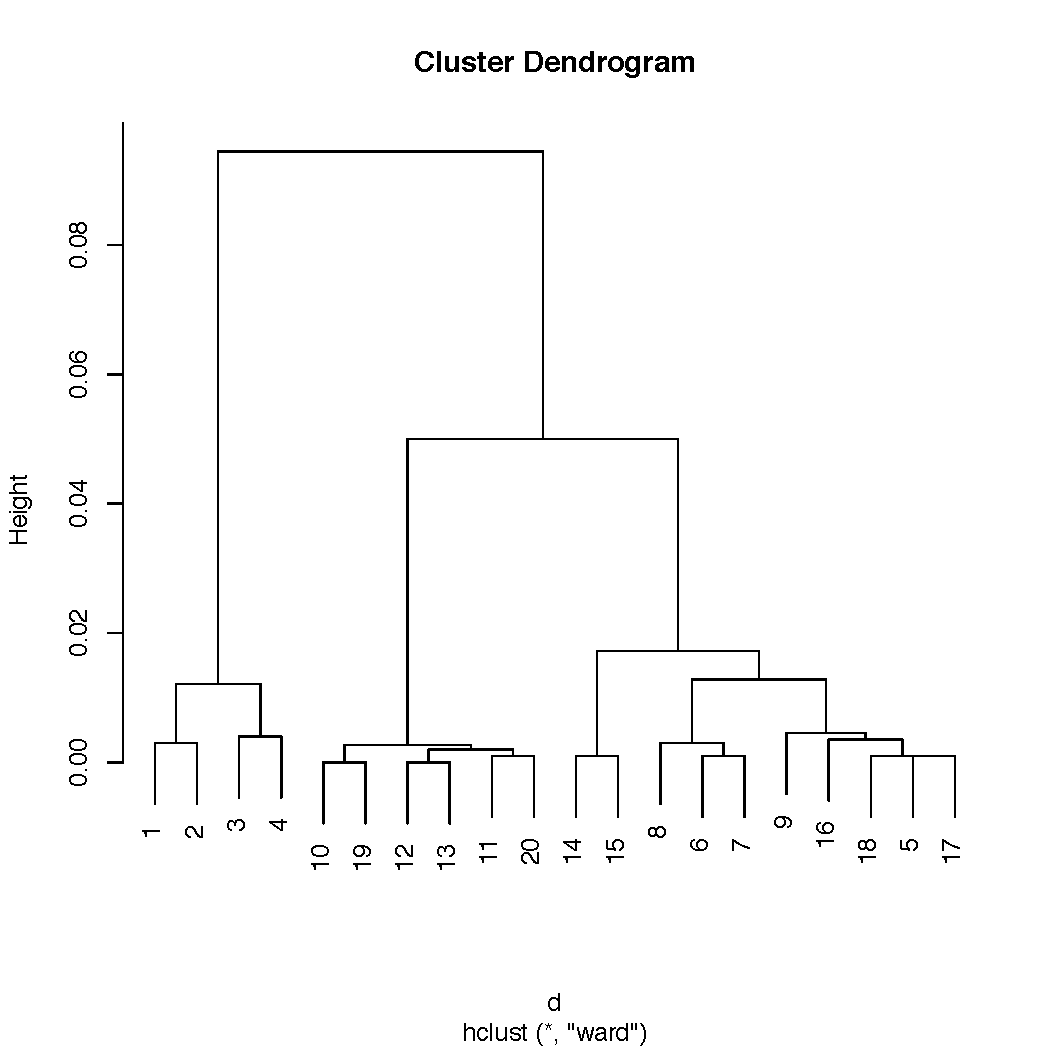
\includegraphics[scale=0.35]{figures/insulin.pdf}
\end{center}
}

\begin{frame}[fragile]
\begin{verbatim}
 No.  Av. CC  I/sig  File Name
   1  0.9796   2.25 NATIVE_SWEEP11.HKL
   2  0.9822   3.61 NATIVE_SWEEP22.HKL
   3  0.9807   7.49 NATIVE_SWEEP33.HKL
<snip>
  18  0.9925   2.64 NATIVE_SWEEP9.HKL
  19  0.9930   1.69 NATIVE_SWEEP10.HKL
  20  0.9826   3.39 NATIVE_SWEEP12.HKL
\end{verbatim}
\end{frame}

\frame{
\frametitle{Interpretation}
\begin{itemize}
\item{$d = \frac{1}{CC} - 1$}
\item{$CC = \frac{1}{d + 1}$}
\item{$CC = 0.95 \rightarrow d < 0.05$}
\item{Up to you to decide on your limits... at least you know what
    they mean}
\end{itemize}
}

\frame{
\frametitle{Interpretation}
\begin{center}
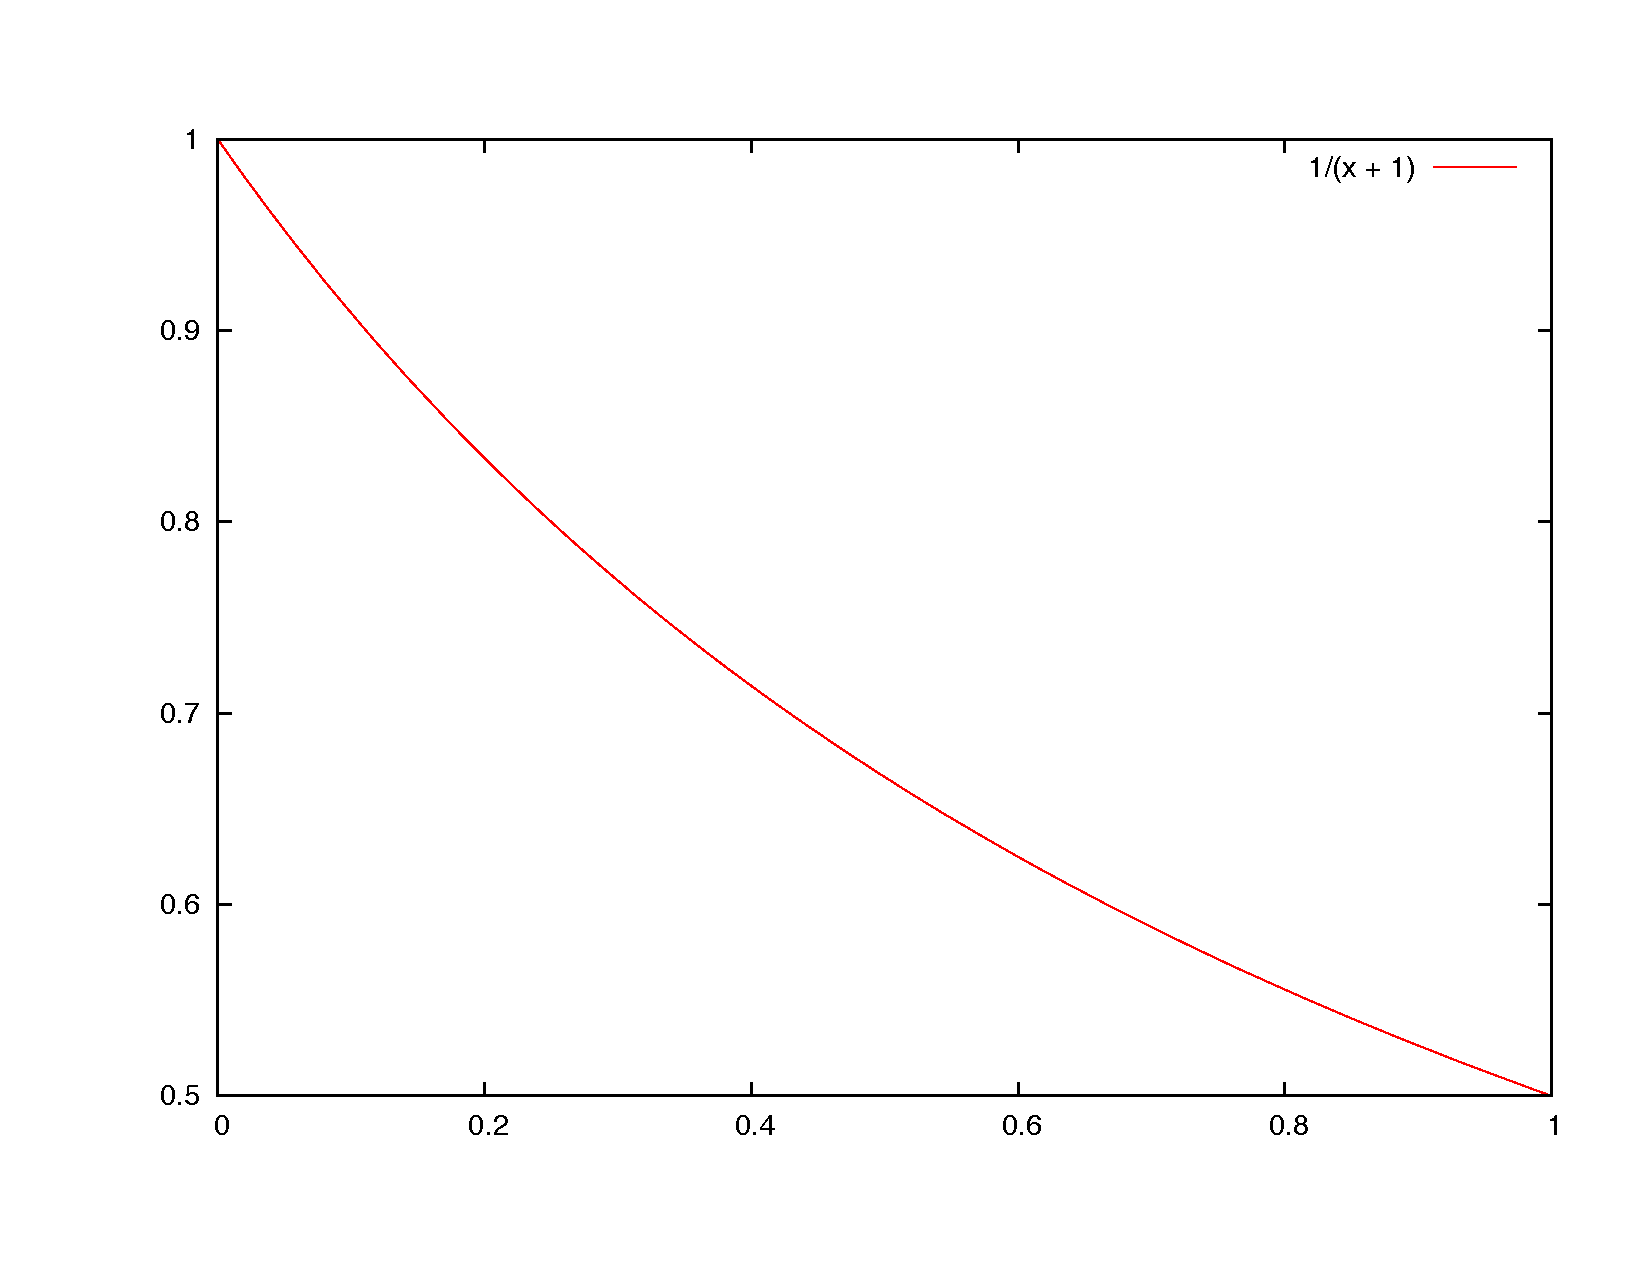
\includegraphics[scale=0.35]{figures/cc_d.pdf}
\end{center}
}

\frame{
\frametitle{Next steps}
\begin{itemize}
\item{Book keeping - take the sweeps you wish to merge from dendogram}
\item{Edit xinfo file}
\item{Run again}
\item{This needs automating, and also calculations performing to tell
    you how complete results will be}
\end{itemize}
}

\frame{
\frametitle{Trivial example - Thaumatin}
\begin{itemize}
\item{Split 450 image Thaumatin data set into 5 x 90 image chunks}
\item{Process as usual, very good results and grouping comes in data
    collection order}
\item{Distances are fantastically small indicating very high CC's}
\end{itemize}
}

\frame{
\frametitle{Results}
\begin{center}
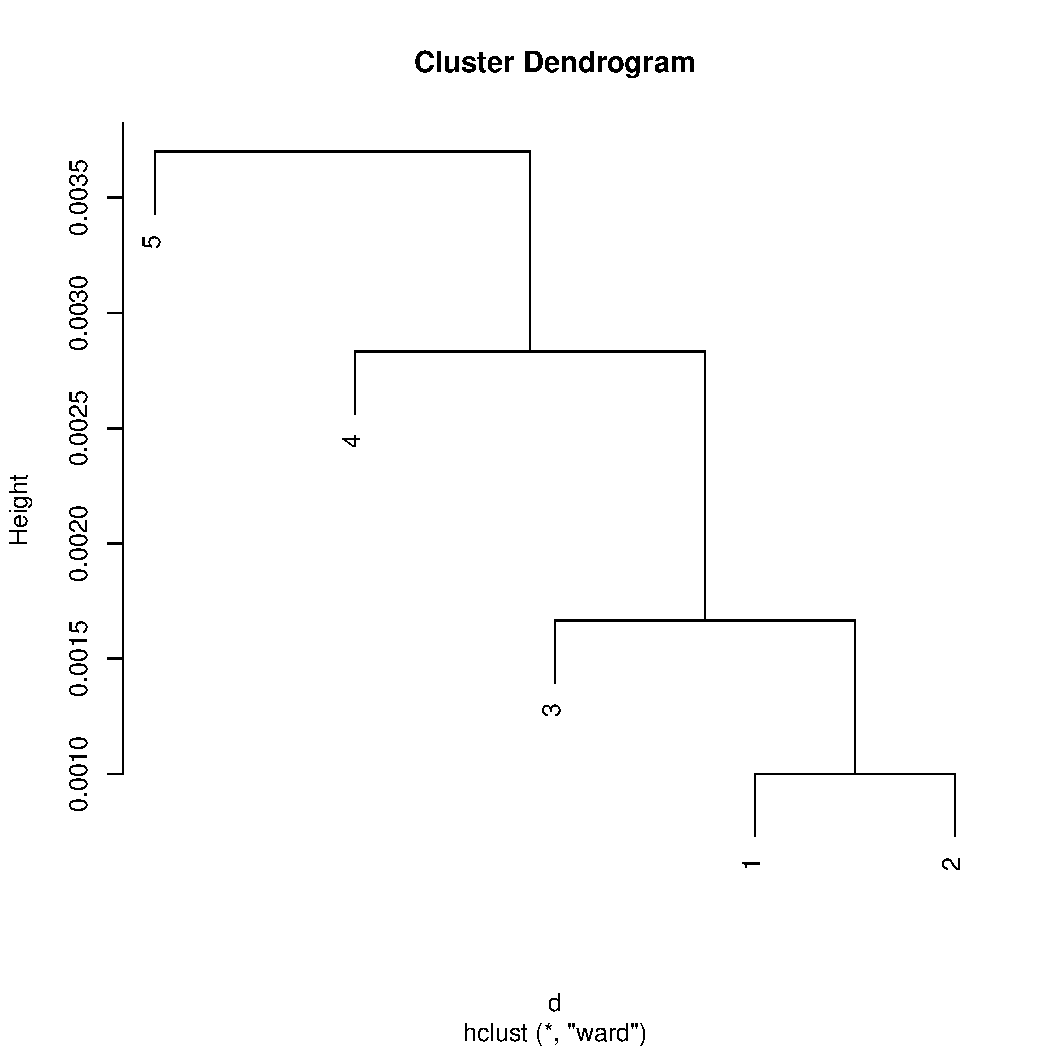
\includegraphics[scale=0.35]{figures/thaumatin.pdf}
\end{center}
}

\frame{
\frametitle{Developments planned from mid April}
\begin{itemize}
\item{Apply to more cases}
\item{Work on clustering}
\item{Include comparison of $R_{\rm{merge}}$ as a function of batch number}
\item{Work on incorporating radiation damage: split sweeps into blocks}
\item{Automate analysis, also allowing for completeness}
\end{itemize}
}

\frame{
\frametitle{Other developments}
\begin{itemize}
\item{Development of xia2 for small molecule crystallography}
\item{Support for complex experimental geometry from imgCIF data}
\item{Full scaling model search with scaling with Aimless and Scala}
\end{itemize}
}

\end{document}
